\section{Logit models for qualitative predictors}\label{sec:logist-qual}

Logistic regression can be generalized to include discrete
explanatory variables, and such models are often called
\glossterm{logit models}.
The main differences (using \PROC{LOGISTIC}) are:

\begin{itemize*}
\item the data are often entered in frequency form, with one observation
       per ``group'', defined by the value(s) of the discrete predictors.
		 With quantitative predictors, the data \emph{must} be entered in
		 \IX{case form}.
\item the discrete predictors must be represented by dummy (0/1) variables
for \PROC{LOGISTIC},
so explanatory variables often need to be recoded.%
\footnote{The \proc{GENMOD} provides a \stmt{CLASS}{GENMOD}, so no
recoding is necessary. The \macro{DUMMY} (\macref{mac:dummy}) may be used
to create the dummy variables for \PROC{LOGISTIC}.}
\item the statistics for goodness-of-fit are computed differently.

\item the \ODS\ used for plotting contains one observation
 per group when the data are in frequency form.
\end{itemize*}

When \emph{all} predictors are discrete, the data actually comprise
a contingency table, and there is a close connection between logit
models and \loglin\ models discussed in \chref{ch:loglin},
so that the methods of that chapter may also be used to analyse the data
presented here. 

Consider the data below, which represents the contingency table for
the arthritis data (\exref{ex:arthrit1})
classified by sex and treatment, ignoring the age variable for the moment.  For each group, the observed probabilities and logits
may be found, as displayed in \tabref{tab:arthlogit3}.
\begin{verbatim}
                        Improvement
  Sex   Treatment    None    Some/Marked     Total

   F     Active        6         21            27
   F     Placebo      19         13            32

   M     Active        7          7            14
   M     Placebo      10          1            11
\end{verbatim}
\begin{table}[htb]
 \caption{Arthritis data, by sex and treatment}\label{tab:arthlogit3}
 \begin{center}
 \begin{tabular}{|ll|rrrrr|}
 \hline
      &           & Number &       & Observed &   Odds & Observed \\
  Sex & Treatment & Better & Total & Pr\{better\} & Better & Logit \\ 
   \hline 
  Female & Active & 21 & 27 & 0.7778 & 3.50 & 1.2529 \\ 
  Female & Placebo & 13 & 32 & 0.4062 & 0.68 & -0.3797 \\ 
  Male & Active & 7 & 14 & 0.5000 & 1.00 & 0.0000 \\ 
  Male & Placebo & 1 & 11 & 0.0909 & 0.10 & -2.3026 \\ 
 \hline
 \end{tabular}
 \end{center}
\end{table}


A simple model might assume additive (``main'') effects
for sex and treatment on the log odds of improvement,
of the same form as model \eqref{eq:logit1}.
\begin{equation} \label{eq:logst}
  \logit \,  ( \pi_{ij} ) = \alpha   +
  \beta _1 \,  x_1  +
  \beta _2 \,  x_2
  \period
\end{equation}
In this model,
\begin{itemize}

\item \(x_1\) and \(x_2\) are dummy (0/1) variables representing sex and
       treatment, respectively.  They are defined as 
\begin{equation*}
 x_1 = \left\{
    \begin{array}{ll}
    0  & \mbox{ if male} \\
    1  & \mbox{ if female}
    \end{array}
    \right.
 \qquad\qquad
 x_2 = \left\{
    \begin{array}{ll}
    0  & \mbox{ if placebo} \\
    1  & \mbox{ if active}
    \end{array}
    \right.
\end{equation*}
\item \(\alpha\) is the log odds of improvement for the baseline group
with $x_1=0$ and $x_2=0$---males receiving
the placebo.

\item \(\beta_1\) is the increment in log odds for being female
as opposed to male.
Therefore, \(e^{ \beta_1 }\) gives the odds of improvement
for females relative to males.

\item \(\beta_2\) is the increment in log odds for being in the
active treatment group.  \(e^{ \beta_2 }\) gives the odds of
improvement for the active treatment group relative to
placebo.

\end{itemize}

Thus, the parameters defined here are \emph{incremental effects}.  The
intercept corresponds to a baseline group (males given the placebo);
the other parameters are incremental effects for the other groups
compared to the baseline group.
Thus, when \(\alpha\), \(\beta _1\), and \(\beta _2\) have
been estimated, the fitted logits and predicted odds are:

\begin{center}
\vspace{1ex}
{\renewcommand{\arraystretch}{1.2}
\begin{tabular}{|ll|cc|}
\hline
Sex  &  Treatment & Logit & Odds Improved  \\[.5ex] \hline

Female & Active & \(\alpha + \beta_1 + \beta_2\) & \(e^{\alpha + \beta_1 + \beta_2}\)  \\
Female & Placebo & \(\alpha + \beta_1 \) & \(e^{\alpha + \beta_1 }\) \\
Male   & Active  & \(\alpha + \beta_2 \) & \(e^{\alpha + \beta_2 }\) \\
Male  & Placebo  & \(\alpha \) & \(e^{\alpha}\) \\ \hline
\end{tabular}
}
\end{center}

In general, there may be any number of explanatory variables, as in multiple
regression.  A discrete predictor with $c$ categories may be represented
by  $c-1$ dummy variables.  Interactions between predictors may be included
in the model by defining interaction variables as products of the main effect variables, as with \PROC{REG}.
For example, the interaction of sex and treatment could be included in the
model \eqref{eq:logst} by adding a term
$\beta_3 x_3$, where $x_3 = x_1 \times x_2$.%
\footnote{In the current example, this would give a saturated model,  which would
necessarily fit perfectly.
We usually try to obtain the simplest model with an adequate fit.}

\begin{Example}[arthrit8]{Arthritis treatment}
The following \Dstp\ creates a \Dset\ in frequency form
named \pname{ arthrit}.  The dummy variables \verb|_SEX_| and \verb|_TREAT_|
corresponding to \(x_1\) and \(x_2\) are created with logical assignment
statements, 
as is the
dichotomous response variable, \pname{ better}.

The first logistic regression model includes effects for sex and
treatment, specified by the dummy variables in the \stmt{MODEL}{LOGISTIC}.
Again,
the \opt{descending}{LOGISTIC} is used
so that predicted results will be for
Pr\{better=1\}.

\begin{listing}
data arthrits;
   input sex$ trtment$ improve$ count;
   _treat_ = (trtment='Active');
   _sex_   = (sex='F');
   better  = (improve='some');
datalines;
F Active  none   6
M Active  none   7
F Active  some  21
M Active  some   7
F Placebo none  19
M Placebo none  10
F Placebo some  13
M Placebo some   1
;
proc logistic data=arthrits descending;
   freq count;
   model better = _sex_ _treat_ / scale=none aggregate;
\end{listing}
The options \pname{scale=none aggregate} provide goodness of fit tests%
\glosstex{goodness-of-fit}
for the model.  The goodness of fit tests are based on the difference
between the actual model fitted and the saturated model (containing
an interaction of sex and treatment in this example), which would fit
perfectly.  The results shown in \outref{out:glogist0.1} are produced.
\begin{Output}[htb]
\caption{Arthritis treatment data: Overall tests}\label{out:glogist0.1}
\small
\verbatiminput{ch6/out/glogist0.1}
\end{Output}
The Chi-square tests for BETA=0 in \outref{out:glogist0.1} test the joint effect of sex
and treatment.  Individual effects in the model are tested by Wald
\ix{Wald test}
\(\chi^2\)s, the squared ratio of each parameter divided by its
standard error.  These tests, in \outref{out:glogist0.2}, indicate that both sex and
treatment effects are highly significant.

\begin{Output}[htb]
\caption{Arthritis treatment data: Parameter estimates}\label{out:glogist0.2}
\small
\verbatiminput{ch6/out/glogist0.2}
\end{Output}
The fitted model,

\begin{equation} \label{eq:fitmod}
  \logit ( \pi_{ij} ) = -1.90  +  1.47 \, \mbox{sex}
  +  1.78 \, \mbox{treat}
\end{equation}
is most easily interpreted by considering the odds ratios
corresponding to the parameters:

\begin{itemize}

\item 1.47 is the increment to log odds of a better outcome for
       females; the \IX{odds ratio} \(e^{1.47} = 4.34\) indicates that
       females are 4.3 times as likely to achieve a better outcome
       than males.

\item 1.78 is the increment to log odds for the treatment group; the
       odds ratio \(e^{1.78} = 5.94\) indicates that the treated
       group is nearly 6 times as likely to achieve a better outcome
       than the placebo group.

\end{itemize}
\end{Example}

\subsection{Plotting results from \PROC{LOGISTIC}}\label{sec:qual-plots}
As we saw in \secref{sec:logist-quantp}, you can save predicted probabilities and fitted logits in an
\ODS\ which may be used for plotting and visualizing the results.

\begin{Example}[arthrit9]{Arthritis treatment}
Adding an \stmt{OUTPUT}{LOGISTIC} to the \PROC{LOGISTIC} step produces a \Dset\ containing estimated
logit values for each group, and corresponding predicted
probabilities of improvement and confidence limits (\pname{UPPER}, \pname{LOWER}) for these probabilities.

\begin{listing}
proc logistic data=arthrits;
   freq count;
   format better outcome.;
   model better = _sex_ _treat_;
   \textbf{output out=results p=predict l=lower u=upper xbeta=logit;}
proc print data=results;
   id sex trtment; var improve count predict lower upper logit;
   format predict lower upper logit 7.3;
\end{listing}
The \ODS\ \pname{RESULTS} is shown in \outref{out:glogist0.3}.
There are two observations for each group (for none and some
improvement).  The \pname{PREDICT} variable gives the predicted
probability of an improved outcome according to model \eqref{eq:fitmod}, using the
inverse transformation \eqref{eq:logit3} of logit to probability.
Note that the fitted statistics are the same for both observations
corresponding to each sex-treatment combination.
\begin{Output}[htb]
\caption{Arthritis treatment data: \pname{RESULTS} \Dset}\label{out:glogist0.3}
\small
\verbatiminput{ch6/out/glogist0.3}
\end{Output}

To plot the predicted probabilities of improvement and confidence
limits from the \pname{RESULTS} \Dset, we select the observations
for \pname{improve='some'}.  A plot can be done as a bar chart with \PROC{GCHART},
or as a line graph with \PROC{GPLOT}.  Confidence limits can be
added to either with the SAS/GRAPH Annotate facility.  The statements
below show how a grouped horizontal bar chart (see \figref{fig:glogist0})
is constructed.
\begin{listing}
data results;
   set results;
   if improve='some';
   label predict='Prob. Improved';
data limits;
   set results;
   xsys='2'; ysys='2';
   midpoint=trtment;
   group=sex; when='A'; position='+';
   x = lower;  function='MOVE   '; output;
   text='|';   function='LABEL  '; output;
   x = upper;  function='DRAW   '; output;
   text='|';   function='LABEL  '; output;

proc gchart data=results;
   hbar trtment / sumvar=predict group=sex gspace=3
                  patternid=midpoint
                  anno=limits
                  raxis=axis1
                  maxis=axis2
                  gaxis=axis3;
   axis1 order=(0 to 1 by .2) minor=none
         label=(h=1.5) value=(h=1.3);
   axis2 label=(h=1.3 'Treat') value=(h=1.1);
   axis3 label=(h=1.3) value=(h=1.2);
   pattern1 v=solid c=cyan;
   pattern2 v=solid c=rose;
\end{listing}
\begin{figure}[!htb]
  \centering
  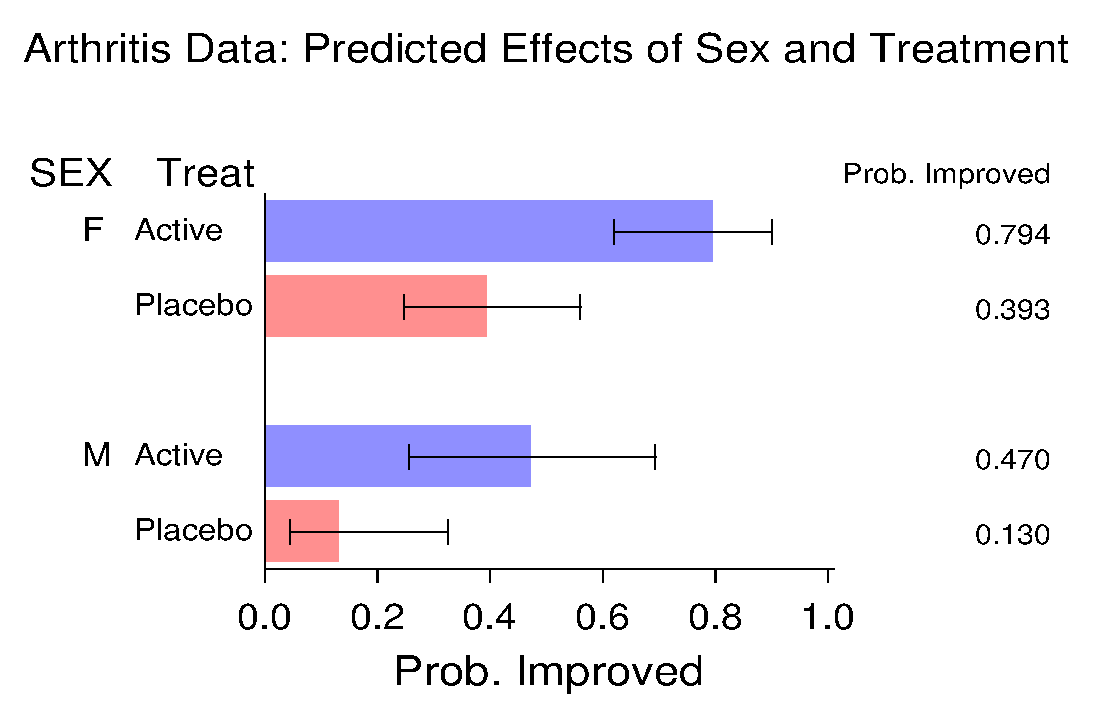
\includegraphics[scale=.7,clip]{ch6/fig/glogist0}
  \caption{Predicted probabilities of improvement}\label{fig:glogist0}
\end{figure}

Alternatively, you may prefer a line graph to a bar chart.
\figref{fig:glogist11} shows one example, with separate lines
for the two treatment groups.
The observed probabilities of improvement are shown by dots;
these values were calculated from the \pname{COUNT} variable
in the \pname{RESULTS} \Dset.
The plotting steps are not shown here to conserve space.
\begin{figure}[!htb]
  \centering
  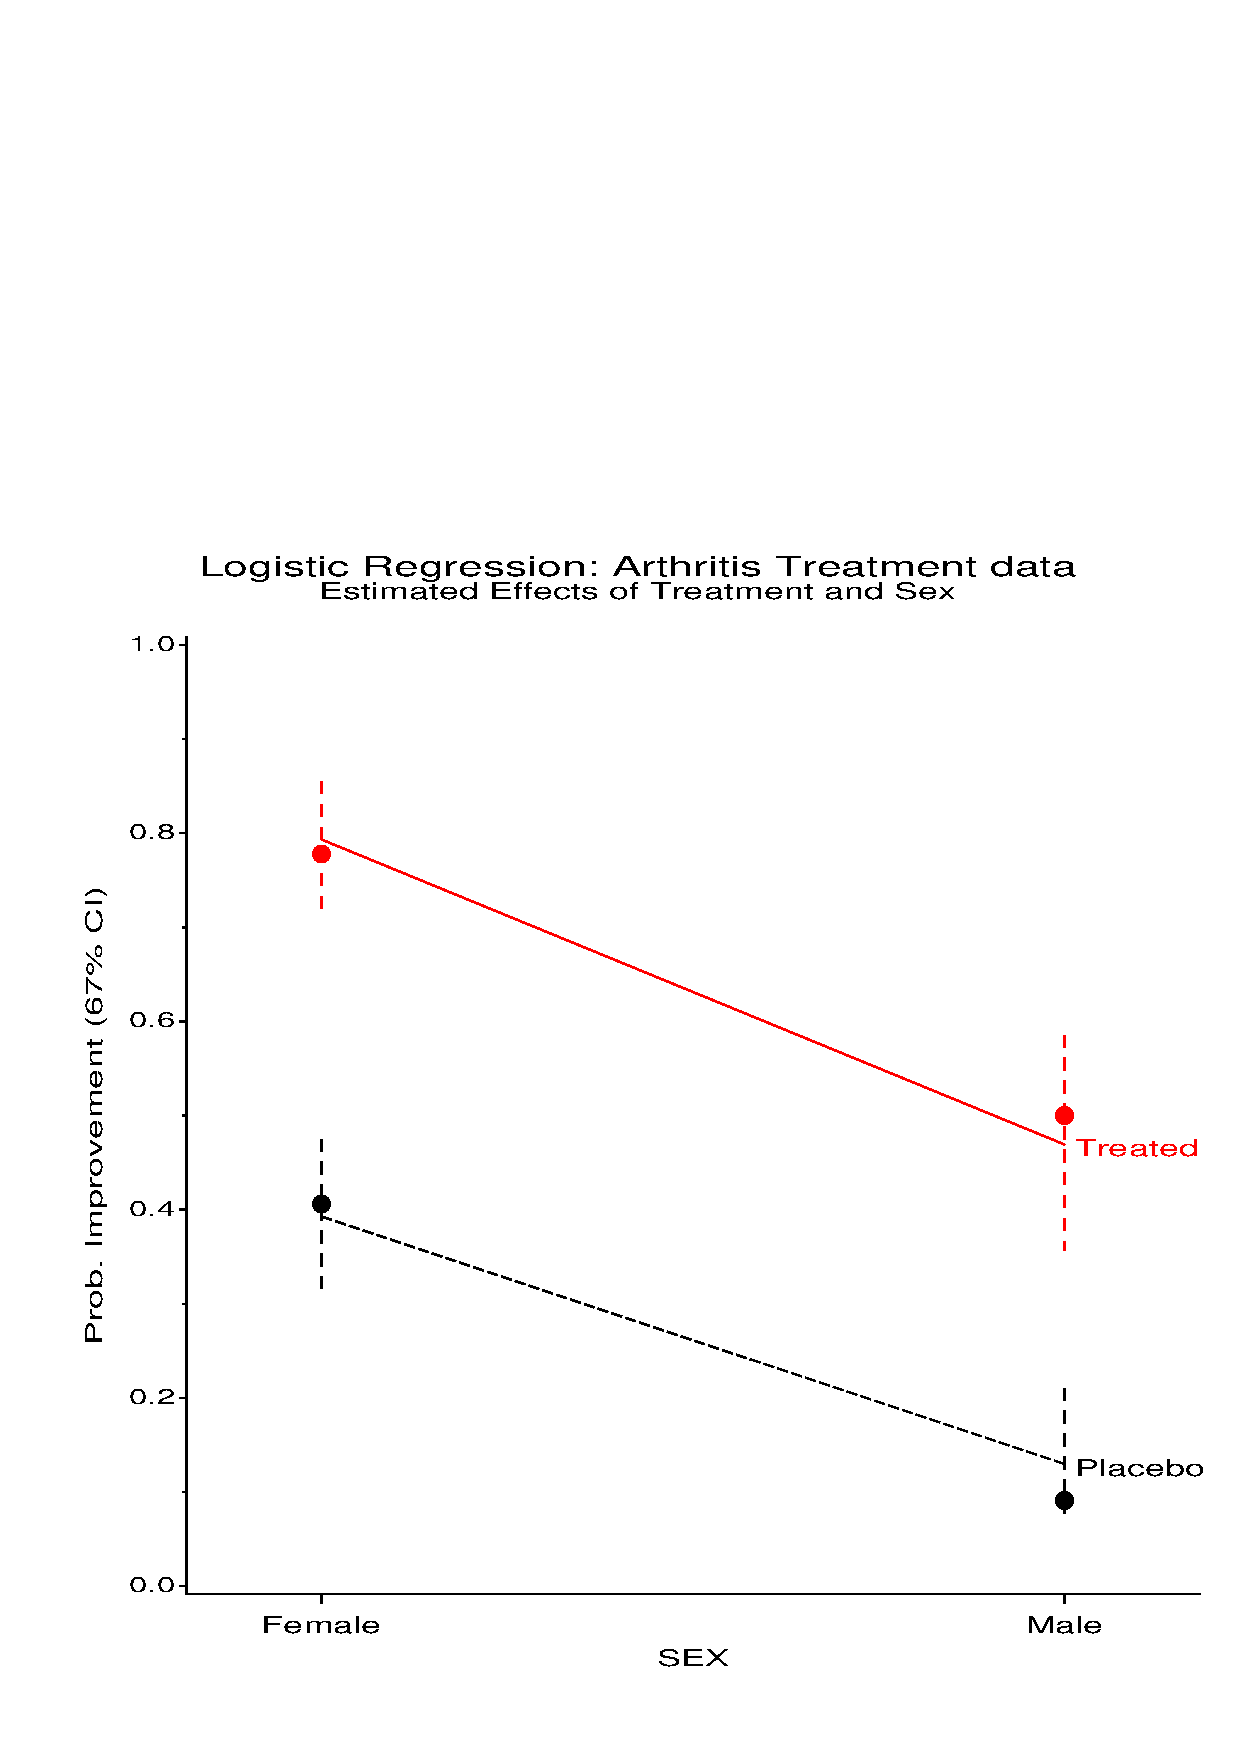
\includegraphics[scale=.7]{ch6/fig/glogist11}
  \caption{Line graph of observed and predicted probabilities}\label{fig:glogist11}
\end{figure}
\end{Example}
 
